\section{Model}

\subsection{Root Geometry}

This paper uses a vertex-based model. Edges and vertices form the cell wall, and the area enclosed by these edges represent the cytoplasm. Because the cell wall has a different diffusion rate than the cytoplasm \cite{kramer2007}, all of the vertexes, edges, and interior regions contain hormones.

\usetikzlibrary{decorations}
\usetikzlibrary{shapes.arrows}
\usetikzlibrary{arrows, arrows.meta}

\begin{center}
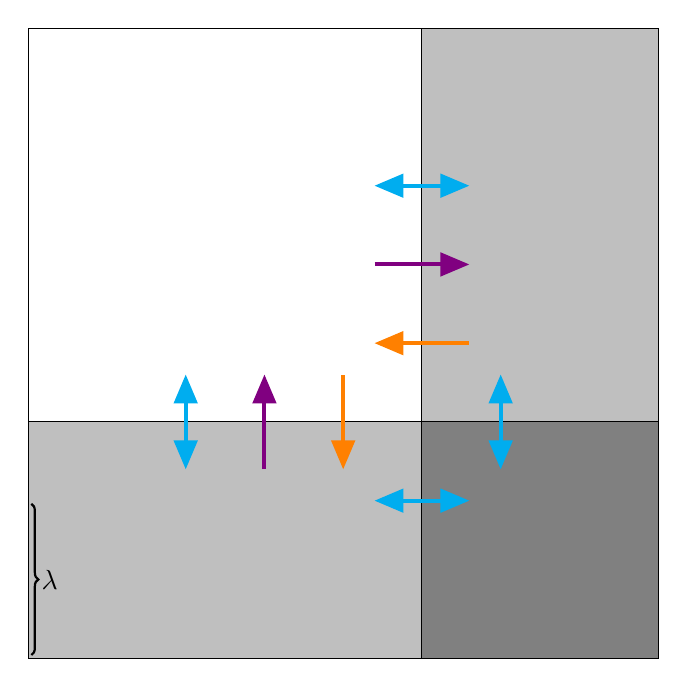
\begin{tikzpicture}[scale=2]

\draw (0,0) -- (4,0) -- (4,4) -- (0,4) -- cycle;
\draw[fill = lightgray] (0, 0) rectangle (3, 1.5);
\draw[fill = lightgray] (2.5, 1.5) rectangle (4, 4);
\draw[fill = gray] (2.5, 0) rectangle (4, 1.5);
\draw[thick, decorate, decoration={brace, mirror}] (0.02,0.02) -- node[right] {$\lambda$} (0.02, 0.98);


\draw[thick, draw = cyan, >=triangle 45, <->, line width = 0.5mm] 
	(1, 1.2) -- ++(0, 0.6);
\draw[thick, draw = violet, >=triangle 45, ->, line width = 0.5mm]
	(1.5, 1.2) -- ++(0, 0.6);
\draw[thick, draw = orange, >=triangle 45, <-, line width = 0.5mm] 
	(2, 1.2) -- ++(0, 0.6);

\draw[thick, draw = cyan, >=triangle 45, <->, line width = 0.5mm] 
	(2.2, 3) -- ++(0.6, 0);
\draw[thick, draw = violet, >=triangle 45, ->, line width = 0.5mm] 
	(2.2, 2.5) -- ++(0.6, 0);
\draw[thick, draw = orange, >=triangle 45, <-, line width = 0.5mm] 
	(2.2, 2) -- ++(0.6, 0);

\draw[thick, draw = cyan, >=triangle 45, <->, line width = 0.5mm] 
	(3, 1.2) -- ++(0, 0.6); 
\draw[thick, draw = cyan, >=triangle 45, <->, line width = 0.5mm] 
	(2.2, 1) -- ++(0.6, 0); 

\end{tikzpicture}
\end{center}
